\section{Lineare Abbildungen}
$A: \mathbb{R}^{2} \rightarrow \mathbb{R}^{2}$ heißt linear, wenn für jedes $a,b \in \mathbb{R}^{2}$ gilt: $A(x\vec{a} + y \vec{b})=xA(\vec{a}) + yA(\vec{b})$\\

$A\begin{pmatrix} 1\\0 \end{pmatrix}$ und $A\begin{pmatrix} 0 \\ 1 \end{pmatrix}$ können beliebig vorgegeben werden. Anderseits ist $A$ durch diese bestimmt.\\

$A\begin{pmatrix} x \\ y \end{pmatrix}= x\cdot A\begin{pmatrix} 1 \\ 0 \end{pmatrix} + y \cdot A\begin{pmatrix} 0 \\ 1 \end{pmatrix}$ \\

$A\begin{pmatrix}1 \\ 0 \end{pmatrix} = \begin{pmatrix} a_{1} \\ a_{2} \end{pmatrix} \qquad A\begin{pmatrix} 0 \\ 1 \end{pmatrix} = \begin{pmatrix} b_{1} \\ b_{2} \end{pmatrix}$ \\

$A\begin{pmatrix} x \\ y \end{pmatrix} = \mathop{\underbrace{\begin{pmatrix} a_{1} & b_{1} \\ a_{2} & b_{2} \end{pmatrix}}}\limits_{(2\times 2) - \textrm{Matrix}} \cdot \begin{pmatrix} x \\ y \end{pmatrix} \coloneq \begin{pmatrix} a_{1}x + b_{1} y \\ a_{2}x + b_{2}y\end{pmatrix} = xa+by$\\
Eigenschaft: Die erste Spalte von $A$ ist ist der Bildvektor von $\begin{pmatrix}1 \\ 0 \end{pmatrix}$
%
%
%
\subsubsection{Beispiel: }
$\begin{pmatrix} 1 & 0 \\ 0 & 1 \end{pmatrix}$ repräsentiert die identische Abbildung.
%
%
%
\subsubsection{Satz: }
sind $A,B: \mathbb{R}^{2}\rightarrow \mathbb{R}^{2}$ linear, so auch die Verknüpfung $A \circ B$.
%
%
%
\subsubsection{Beweis:}
$A(B(xa+yb))=A(xB(a)+yB(b))=xAB(a)+yAB(b)$\\
Komposition linearer Abbildungen:\\
$A=\begin{pmatrix} a_{1} & b_{1} \\ a_{2} & b_{2} \end{pmatrix}; \ B=\begin{pmatrix} c_{1} & d_{1} \\ c_{2} & d_{2} \end{pmatrix}$ \\
$A \circ B \ \begin{pmatrix}x_{1} \\ x_{2} \end{pmatrix} = \begin{pmatrix}a_{1} & b_{1} \\ a_{2} & b_{2} \end{pmatrix} \cdot \begin{pmatrix} c_{1}x_{1} + d_{1} x_{2} \\ c_{2}x_{1} + d_{2}x_{2} \end{pmatrix} = \begin{pmatrix} a_{1}c_{1}x_{1} + a_{1}d_{1}x_{2} & b_{1}c_{1}x_{1} + b_{1}d_{1}x_{2} \\ a_{2}c_{1}x_{1} + a_{2}d_{1}x_{2} & b_{2}c_{2}x_{1} + b_{2} d_{2}x_{2} \end{pmatrix} = \begin{pmatrix} a_{1} c_{1} + c_{2} b_{1} & a_{1} d_{1} + b_{1} d_{2} \\ a_{2} c_{1} + b_{2} c_{2} & a_{2}d_{1} + b_{2}d_{2} \end{pmatrix} \ \begin{pmatrix} x_{1} \\ x_{2} \end{pmatrix}$\\
\qquad\\
\qquad\\
$\begin{pmatrix} \textcolor{pred}{a_{1}} & \textcolor{pred}{b_{1}} \\ \textcolor{pviolet}{a_{2}} & \textcolor{pviolet}{b_{2}}\end{pmatrix} \cdot \begin{pmatrix} \textcolor{pgreen}{c_{1}} & \textcolor{pblue}{d_{1}} \\ \textcolor{pgreen}{c_{2}} & \textcolor{pblue}{d_{2}}\end{pmatrix} = \begin{pmatrix}\textcolor{pred}{a_{1}}\textcolor{pgreen}{c_{1}} + \textcolor{pred}{b_{1}}\textcolor{pgreen}{c_{2}}  & \textcolor{pred}{a_{1}}\textcolor{pblue}{d_{1}} + \textcolor{pred}{b_{1}}\textcolor{pblue}{d_{2}} \\ \textcolor{pviolet}{a_{2}}\textcolor{pgreen}{c_{1}}+\textcolor{pviolet}{b_{2}}\textcolor{pgreen}{c_{2}} & \textcolor{pviolet}{a_{2}} \textcolor{pblue}{d_{1}} + \textcolor{pviolet}{b_{2}}\textcolor{pblue}{d_{2}}\end{pmatrix}$\\
\qquad\\
\begin{figure}[H]
	\centering
	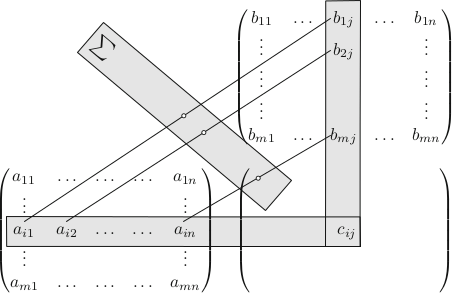
\includegraphics[width=0.5\textwidth]
	{mainmatter/chapter1/pics/matrixmult.png}
	\caption{Schema der Matrixmultiplikation} 
\end{figure}
Matrixmultiplikation entspricht Komposition von Abbildungen\\
Sie ist im Allgemeinen nicht Kommutativ.\\
\qquad\\
$\begin{pmatrix} 1 & 2 \\ 3 & 4 \end{pmatrix} \cdot \begin{pmatrix} 5 & 6 \\ 7 & 8 \end{pmatrix} = \begin{pmatrix} 1 \cdot 5 + 2 \cdot 7 & 1 \cdot 6 + 2 \cdot 8 \\ 3 \cdot 5 + 4 \cdot 7 & 3 \cdot 6 + 4 \cdot 8\end{pmatrix} = \begin{pmatrix} 19 & 22 \\ 43 & 50 \end{pmatrix}$ \\
.\qquad \qquad \qquad \qquad \qquad \qquad \qquad$ \neq $\\
$\begin{pmatrix} 5 & 6 \\ 7 & 8 \end{pmatrix} \cdot \begin{pmatrix} 1 & 2 \\ 3 & 4 \end{pmatrix}= \begin{pmatrix} 5 \cdot 1 + 6 \cdot 3 & 5 \cdot 2 + 6 \cdot 4 \\ 7 \cdot 1 + 8 \cdot 2 & 7 \cdot 2 + 8 \cdot 4 \end{pmatrix} = \begin{pmatrix} 23 & 34 \\ 23 & 46 \end{pmatrix}$\\
%
%
%
\subsubsection{Satz:}
Matrixmultiplikation ist assoziativ.
%
%
%
\subsubsection{Beweis:} 
$(A\cdot B) \cdot C = A \cdot (B \cdot C)$ \\
Interpretiere $A,B,C$ als Abbildungen\\
$A\circ (B \circ C) (a) = A\circ B (C(a)) = A(B(C(a)))$\\
$(A\circ B) \circ C (a)=(A\circ B)C(a)=A(B(C(a)))$
%
%
%
\subsubsection{Satz:}
$A: \mathbb{R}^{2} \rightarrow \mathbb{R}$ lineare Abbildungen\\
$A$ ist injektiv $\Leftrightarrow A$ ist surjektiv
%
%
%
\subsubsection{Beweis:}
$Ax=b$ \\
Existenz von $x \Leftrightarrow$ Surjektivität\\
Eindeutigkeit von $x \Leftrightarrow$ Injektivität\\
$det A \neq 0 \Leftrightarrow A$ injektiv $\Leftrightarrow A$ surjektiv. \\
/* Durch Benutzung der Cramerschen Regel */